\chapter{Architecture Overview}
	Democritus' compiler is built off of Professor Stephen Edwards' \texttt{MicroC} compiler. 
   
   \begin{center}
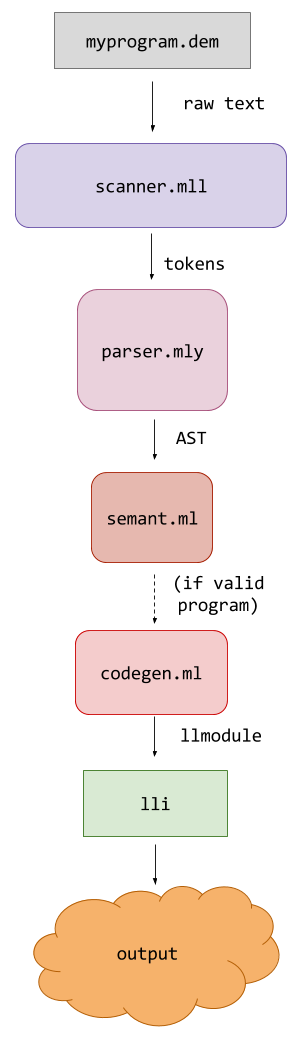
\includegraphics[width=.25\textwidth]{img/flow_chart.png}
  \end{center}
  \newpage

\section{Compiler Overview}
  Several files make up the source code of the compiler. These include:
  \begin{itemize}
    \item \texttt{scanner.mll}: the OCamllex scanner.
    \item \texttt{ast.ml}: the abstract syntax tree, summarizing the overall structure of a Democritus program. 
    \item \texttt{parser.mly}: the Ocamlyacc parser. Tokens from the scanner are parsed into the abstract syntax tree in the parser.
    \item \texttt{semant.ml}: the semantic analyzer.
    \item \texttt{codegen.ml}: the LLVM IR code generator.
    \item \texttt{democritus.ml}: the overarching OCaml program that calls the four main steps of the compiler.
    \item \texttt{bindings.c}: a C file that provides facilitates low-level operations that interact with the OS through C functions, such as for threads, which is then compiled to LLVM bytecode.
  \end{itemize}
	\subsection{The Scanner}
    The scanner is simply a text scanner that parses text into various tokens, to then be interpreted by the parser. The regular expressions used by the scanner are listed in the language reference chapter.

	\subsection{The Parser}
    The parser is a token scanner that converts the tokens read into a valid abstract syntax tree of the program. If the program follows valid syntax, it will be parsed accordingly. Otherwise, compilation of code will yield a parse error. The structure of the program is as follows:

	\subsection{The Semantic Analyzer}
	The semantic analyzer checks the consistency and correctness of user programs. For example, it will check whether variables are defined within a scope, whether types of expressions match their uses in definitions and function calls, and whether structs are used correctly (a large modification we made was semantic checking for circular struct definitions).  

	\subsection{The Code Generator}
	The code generator then takes in a definition of a program and builds the equivalent LLVM IR. 